\documentclass[../../main.tex]{subfiles}

\graphicspath{{../../image/}{../../figure/}}

\begin{document}

\section{得分匹配}\label{section:ch20-得分匹配}

截至目前，本章讨论的去噪扩散模型与另一类相对独立发展的深度生成式模型密切相关，它们都基于\textbf{得分匹配}（score matching）（Hyvärinen, 2005; Song and Ermon, 2019）。这些模型利用的得分函数（或 Stein 得分）则定义为对数似然函数关于数据向量 $\bm{x}$ 的梯度：
\begin{align}
\bm{s}(\bm{x})=\nabla_{\bm{x}}\ln p(\bm{x}).
\label{align:ch20-得分}
\end{align}

\begin{definition}[得分函数]\label{definition:ch20-得分函数}
设 $p(\bm{x})$ 关于 $\bm{x}$ 可微且为正。称向量值函数
\begin{align*}
\bm{s}(\bm{x})=\nabla_{\bm{x}}\ln p(\bm{x})
\end{align*}
为分布 $p$ 的\textbf{得分函数}（score function），也称 \textbf{Stein 得分}。若 $p$ 还依赖参数 $\bm{w}$，则记 $\bm{s}(\bm{x},\bm{w})=\nabla_{\bm{x}}\ln p(\bm{x}\mid\bm{w})$。
\end{definition}

% SUPPLEMENT: parent=definition:ch20-得分函数; kind=motivation; location=紧随其后的 remark（重构新增）
\begin{remark}（重构新增）
得分函数是“对数密度关于\emph{数据}的梯度”，与通常“关于参数 $\bm{w}$ 的梯度”完全不同：前者指向“往哪个方向移动 $\bm{x}$ 能使密度增大”，后者指向“怎样调整参数能使似然增大”。这一区分是理解整节的钥匙——训练模型需要后者，而从模型采样需要前者。\par
定义要求 $p>0$ 且可微：否则 $\ln p$ 或其梯度无定义。在支撑集边界附近得分函数可能发散，这是数值实现时要作裁剪或平滑的原因。另外，$\bm{s}(\bm{x})$ 是与 $\bm{x}$ 同维的向量值函数，其第 $i$ 个分量 $s_i(\bm{x})=\partial\ln p(\bm{x})/\partial x_i$ 只与 $\bm{x}$ 的第 $i$ 个分量对应；若 $\bm{x}$ 是图像，$\bm{s}(\bm{x})$ 也可视为同尺寸的“得分图像”。\par
得分函数有一个关键性质：它不依赖归一化常数。若 $p(\bm{x})=\widetilde{p}(\bm{x})/Z$ 且 $Z$ 与 $\bm{x}$ 无关，则 $\nabla_{\bm{x}}\ln p=\nabla_{\bm{x}}\ln\widetilde{p}$。这正是基于能量的模型可以绕开配分函数的原因（参见\cref{subsection:ch14-基于能量的模型}）。
\end{remark}

这里需要强调的是，梯度是针对数据向量 $\bm{x}$ 计算的，而不是针对任何参数向量。注意 $\bm{s}(\bm{x})$ 是一个与 $\bm{x}$ 维度相同的向量值函数，并且其中的每个元素 $s_i(\bm{x})=\partial\ln p(\bm{x})/\partial x_i$ 都与 $\bm{x}$ 的相应元素 $x_i$ 相关联。例如，如果 $\bm{x}$ 是一个图像，那么 $\bm{s}(\bm{x})$ 也可以表示为一个同尺寸的图像，其中对应的像素是图像的得分。\cref{figure:ch20-得分场}显示了二维中的概率密度示例以及相应的得分函数。

\begin{figure}[htbp]
  \centering
  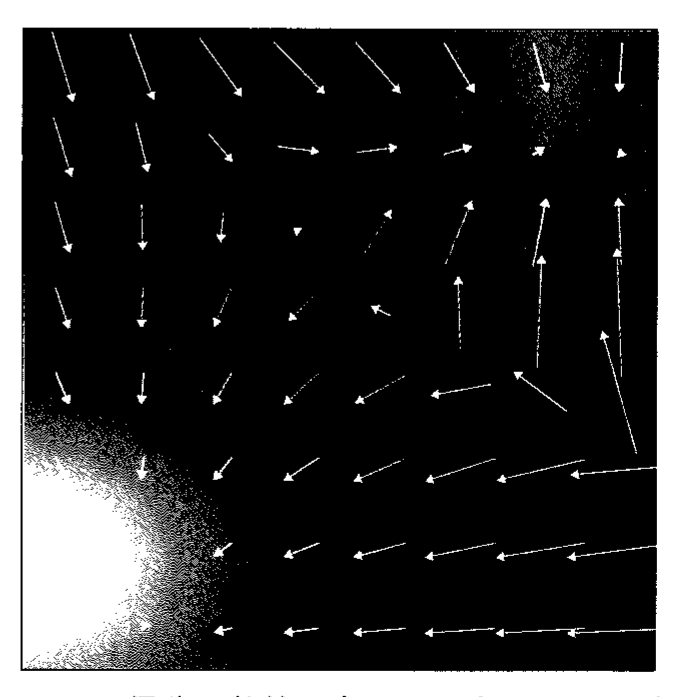
\includegraphics[width=0.42\textwidth]{ch20-fig20-5-score-field.png}
  \caption{得分函数的示意图，图中显示了两种信息的融合：由 Gauss 混合分布构成的二维分布，其作为向量绘制在 $\bm{x}$ 值的规则网格上，表示为热图；以及由\eqref{align:ch20-得分}定义的相应的概率密度示例以及相应的得分函数}
  \label{figure:ch20-得分场}
\end{figure}

为了理解得分函数的用处，考虑两个函数 $q(\bm{x})$ 和 $p(\bm{x})$，它们具有得分相等的属性，所以对于 $\bm{x}$ 的所有值，$\nabla\ln q(\bm{x})=\nabla\ln p(\bm{x})$。我们对这个等式的两边关于 $\bm{x}$ 积分并取指数，则可以得到 $q(\bm{x})=Kp(\bm{x})$，其中 $K$ 是一个独立于 $\bm{x}$ 的常数。所以如果我们能学习到一个得分函数的模型 $\bm{s}(\bm{x},\bm{w})$，就可以重建原始数据分布，所得结果与之前的相比，最多相差一个常数倍数。

\begin{proposition}[得分确定密度至多相差常数倍]\label{proposition:ch20-得分确定密度}
设 $p,q$ 是 $\mathbb{R}^{D}$ 上处处为正的光滑概率密度，且对一切 $\bm{x}$ 有 $\nabla_{\bm{x}}\ln q(\bm{x})=\nabla_{\bm{x}}\ln p(\bm{x})$。则存在常数 $K>0$，使得 $q(\bm{x})=Kp(\bm{x})$ 对一切 $\bm{x}$ 成立。
\end{proposition}

\begin{proof}（重构新增）
令 $h(\bm{x})=\ln q(\bm{x})-\ln p(\bm{x})$。由假设 $\nabla_{\bm{x}}h(\bm{x})=\nabla_{\bm{x}}\ln q(\bm{x})-\nabla_{\bm{x}}\ln p(\bm{x})=\bm{0}$ 对一切 $\bm{x}$ 成立。$\mathbb{R}^{D}$ 连通，梯度处处为零的光滑函数必为常数，故 $h(\bm{x})\equiv\ln K$，即 $q(\bm{x})=Kp(\bm{x})$。又 $p,q>0$，故 $K>0$；若二者都是概率密度，则积分得 $K=1$。证毕。
\end{proof}

% SUPPLEMENT: parent=proposition:ch20-得分确定密度; kind=motivation; location=紧随其后的 remark（重构新增）
\begin{remark}（重构新增）
这条命题说明得分函数唯一确定了密度的\emph{形状}，而不确定其归一化：两个得分相同的密度只差一个正常数因子。这对建模是好事——我们不必计算配分函数就能比较密度的相对高低；但也有代价：仅凭得分无法直接得到归一化的概率值，需要用 Langevin 采样得到样本后再估计归一化常数，或转而使用不需归一化的采样方法。\par
证明中的两个条件不可省：连通性保证“梯度为零”推出“常数”（若定义域分成两个不相连的块，两块上的常数可以不同）；正性保证 $\ln$ 处处有定义。若 $p$ 或 $q$ 在某个区域为零，则得分在该处无定义，命题的表述需要改成“在二者都为正的区域上”。\par
若 $p,q$ 都是归一化密度，则 $K=1$，即得分相同意味着密度相同。这一点常被表述为“得分匹配可以识别分布”，但要注意它依赖“二者都归一化”这一额外信息；只拟合得分而不加归一化约束时，$K$ 是自由的。
\end{remark}

\subsection{得分损失函数}\label{subsection:ch20-得分损失}

为了训练这样的模型，需要定义一个损失函数，用于将模型得分函数 $\bm{s}(\bm{x},\bm{w})$ 匹配到旨在生成数据的分布 $p(\bm{x})$ 的得分函数 $\nabla_{\bm{x}}\ln p(\bm{x})$。这样一个损失函数的例子是计算模型得分和真实得分之间的期望平方误差，其由下式给出：
\begin{align}
J(\bm{w})=\frac{1}{2}\int\big\|\bm{s}(\bm{x},\bm{w})-\nabla_{\bm{x}}\ln p(\bm{x})\big\|^2p(\bm{x})\,\mathrm{d}\bm{x}.
\label{align:ch20-得分损失}
\end{align}

正如我们在讨论基于能量的模型时所看到的（参见\cref{subsection:ch14-基于能量的模型}），得分函数不要求相关的概率密度被归一化，因为归一化常数被梯度算子移除了，所以我们在模型选择上有相当大的灵活性。使用深度神经网络表示得分函数 $\bm{s}(\bm{x},\bm{w})$ 的方法有两种。$\bm{s}$ 的每个元素 $s_i$ 都对应于 $\bm{x}$ 中的一个元素 $x_i$，所以第一种方法是使用一个输入数量和输出数量相同的网络。然而，得分函数定义为标量函数（对数概率密度函数）的梯度，这是一类受限的函数（见\cref{exercise:ch20-14}）。另一种方法是使用一个拥有单一输出的网络 $\phi(\bm{x},\bm{w})$，然后使用自动微分计算 $\nabla_{\bm{x}}\phi(\bm{x},\bm{w})$。然而，这方法需要进行两次反向传播，因此计算成本更高。大多数应用通常采用第一种方法（见\cref{exercise:ch20-15}）。

\subsection{修改得分损失}\label{subsection:ch20-修改得分损失}

损失函数\eqref{align:ch20-得分损失}的一个问题是不能直接最小化，因为我们不知道真实的数据得分 $\nabla_{\bm{x}}\ln p(\bm{x})$。我们所知的只是有限的数据集 $\mathcal{D}=\{\bm{x}_1,\cdots,\bm{x}_N\}$，从中可以构建如下经验分布：
\begin{align}
p_{\mathcal{D}}(\bm{x})=\frac{1}{N}\sum_{n=1}^{N}\delta(\bm{x}-\bm{x}_n).
\label{align:ch20-经验分布}
\end{align}
这里的 $\delta(\bm{x})$ 是 Dirac delta 函数，我们可以将其形象地理解为在 $\bm{x}=\bm{0}$ 处无限高的“尖峰”，它具有以下性质：
\begin{align}
\delta(\bm{x})&=0,\quad \bm{x}\neq\bm{0},
\label{align:ch20-delta零}\\
\int\delta(\bm{x})\,\mathrm{d}\bm{x}&=1.
\label{align:ch20-delta归一}
\end{align}

由于\eqref{align:ch20-经验分布}所示的函数不是 $\bm{x}$ 的可微函数，我们无法计算它的得分。但我们可以通过引入噪声模型来“抹平”数据点并给出密度的平滑、可微表示来解决这个问题，这称为 Parzen 估计器或核密度估计器（参见\cref{subsection:ch03-核密度}），定义如下：
\begin{align}
q_{\sigma}(\bm{z})=\int q(\bm{z}\mid\bm{x},\sigma)\,p(\bm{x})\,\mathrm{d}\bm{x},
\label{align:ch20-Parzen}
\end{align}
其中 $q(\bm{z}\mid\bm{x},\sigma)$ 是噪声核。常见的核选择是 Gauss 核：
\begin{align}
q(\bm{z}\mid\bm{x},\sigma)=\mathcal{N}(\bm{z}\mid\bm{x},\sigma^2\bm{I}).
\label{align:ch20-Gauss核}
\end{align}

此时，我们不再最小化损失函数\eqref{align:ch20-得分损失}，而是使用对应于平滑后的 Parzen 密度的损失函数，形式为
\begin{align}
J(\bm{w})=\frac{1}{2}\int\big\|\bm{s}(\bm{z},\bm{w})-\nabla_{\bm{z}}\ln q_{\sigma}(\bm{z})\big\|^2q_{\sigma}(\bm{z})\,\mathrm{d}\bm{z}.
\label{align:ch20-平滑损失}
\end{align}

一个关键结果是，通过将\eqref{align:ch20-Parzen}代入\eqref{align:ch20-平滑损失}，我们可以将这个损失函数重写为以下等价形式（Vincent, 2011）（见\cref{exercise:ch20-17}）。

\begin{proposition}[去噪得分匹配]\label{proposition:ch20-去噪得分匹配}
设 $q_{\sigma}$ 由\eqref{align:ch20-Parzen}与\eqref{align:ch20-Gauss核}给出。则对任意得分模型 $\bm{s}(\bm{z},\bm{w})$，
\begin{align}
J(\bm{w})=\frac{1}{2}\iint\big\|\bm{s}(\bm{z},\bm{w})-\nabla_{\bm{z}}\ln q(\bm{z}\mid\bm{x},\sigma)\big\|^2q(\bm{z}\mid\bm{x},\sigma)\,p(\bm{x})\,\mathrm{d}\bm{z}\,\mathrm{d}\bm{x}+\mathrm{const},
\label{align:ch20-等价损失}
\end{align}
其中 $\mathrm{const}$ 与网络参数 $\bm{w}$ 无关。
\end{proposition}

\begin{proof}（重构新增）
把\eqref{align:ch20-平滑损失}中的平方项展开：
\begin{align*}
J(\bm{w})=\frac{1}{2}\int\|\bm{s}\|^2q_{\sigma}\,\mathrm{d}\bm{z}-\int\bm{s}\cdot\nabla_{\bm{z}}q_{\sigma}\,\mathrm{d}\bm{z}+\frac{1}{2}\int\|\nabla_{\bm{z}}\ln q_{\sigma}\|^2q_{\sigma}\,\mathrm{d}\bm{z},
\end{align*}
其中第二项用了 $\nabla_{\bm{z}}\ln q_{\sigma}\cdot q_{\sigma}=\nabla_{\bm{z}}q_{\sigma}$。第三项不含 $\bm{w}$，可以并入常数。
第一项：由\eqref{align:ch20-Parzen}，$\int\|\bm{s}\|^2q_{\sigma}\,\mathrm{d}\bm{z}=\iint\|\bm{s}\|^2q(\bm{z}\mid\bm{x},\sigma)p(\bm{x})\,\mathrm{d}\bm{z}\,\mathrm{d}\bm{x}$，与\eqref{align:ch20-等价损失}中平方项的第一部分相同。
第二项：对\eqref{align:ch20-Parzen}求梯度得 $\nabla_{\bm{z}}q_{\sigma}(\bm{z})=\int\nabla_{\bm{z}}q(\bm{z}\mid\bm{x},\sigma)p(\bm{x})\,\mathrm{d}\bm{x}$，于是
\begin{align*}
\int\bm{s}\cdot\nabla_{\bm{z}}q_{\sigma}\,\mathrm{d}\bm{z}&=\iint\bm{s}(\bm{z},\bm{w})\cdot\nabla_{\bm{z}}q(\bm{z}\mid\bm{x},\sigma)p(\bm{x})\,\mathrm{d}\bm{z}\,\mathrm{d}\bm{x}\\
&=\iint\bm{s}(\bm{z},\bm{w})\cdot\nabla_{\bm{z}}\ln q(\bm{z}\mid\bm{x},\sigma)\,q(\bm{z}\mid\bm{x},\sigma)p(\bm{x})\,\mathrm{d}\bm{z}\,\mathrm{d}\bm{x},
\end{align*}
这正是\eqref{align:ch20-等价损失}中交叉项的一半（带负号）。合并三项即得\eqref{align:ch20-等价损失}。证毕。
\end{proof}

% SUPPLEMENT: parent=proposition:ch20-去噪得分匹配; kind=motivation; location=紧随其后的 remark（重构新增）
\begin{remark}（重构新增）
\eqref{align:ch20-等价损失}的意义在于把“与未知的 $\nabla\ln q_{\sigma}$ 比较”换成了“与已知的核得分 $\nabla\ln q(\bm{z}\mid\bm{x},\sigma)$ 比较”，因而损失可以用样本 $\bm{x}_n$ 与人工噪声 $\bm{z}$ 直接计算。这正是“去噪”一词的来源：网络要从被噪声污染的 $\bm{z}$ 中估计出把 $\bm{z}$ 拉回 $\bm{x}$ 的方向。\par
条件方面：交换积分次序要求 $q(\bm{z}\mid\bm{x},\sigma)p(\bm{x})$ 可积（Gauss 核保证这一点）；丢弃的第三项之所以与 $\bm{w}$ 无关，是因为它只含真实密度 $q_{\sigma}$。若两个得分模型在某个 $\bm{z}$ 上给出相同输出，这项对二者的相对大小没有影响，因此不能省掉它去比较不同 $\sigma$ 下的绝对损失值。\par
与扩散模型的联系：若取 $\sigma^2=1-\alpha_t$ 并把核均值改为 $\sqrt{\alpha_t}\,\bm{x}$，就得到前向扩散核，此时\eqref{align:ch20-等价损失}与\eqref{align:ch20-KL噪声}具有相同的最小值（相差常数缩放）。这就是“去噪得分匹配”与 DDPM 训练目标等价的含义。
\end{remark}

用经验分布\eqref{align:ch20-经验分布}代替 $p(\bm{x})$，可以得到
\begin{align}
J(\bm{w})=\frac{1}{2N}\sum_{n=1}^{N}\int\big\|\bm{s}(\bm{z},\bm{w})-\nabla_{\bm{z}}\ln q(\bm{z}\mid\bm{x}_n,\sigma)\big\|^2q(\bm{z}\mid\bm{x}_n,\sigma)\,\mathrm{d}\bm{z}+\mathrm{const}.
\label{align:ch20-经验损失}
\end{align}

对于 Gauss 核\eqref{align:ch20-Gauss核}，得分函数变为
\begin{align}
\nabla_{\bm{z}}\ln q(\bm{z}\mid\bm{x},\sigma)=-\frac{1}{\sigma}\,\bm{\varepsilon},
\label{align:ch20-核得分}
\end{align}
其中 $\bm{\varepsilon}=(\bm{z}-\bm{x})/\sigma\sim\mathcal{N}(\bm{\varepsilon}\mid\bm{0},\bm{I})$ 是标准化噪声。考虑特定的噪声模型\eqref{align:ch20-扩散核}，可以得到
\begin{align}
\nabla_{\bm{z}}\ln q(\bm{z}\mid\bm{x},\sigma)=-\frac{1}{\sqrt{1-\alpha_t}}\,\bm{\varepsilon}.
\label{align:ch20-扩散得分}
\end{align}

由此我们可以看出，损失函数\eqref{align:ch20-等价损失}衡量了神经网络预测与噪声 $\bm{\varepsilon}$ 之间的差异。所以，该损失函数与去噪扩散模型中使用的损失函数\eqref{align:ch20-KL噪声}拥有相同的最小值，得分函数 $\bm{s}(\bm{z},\bm{w})$ 扮演的角色与噪声预测网络 $\bm{g}(\bm{z},\bm{w},t)$ 相同，但前者做了常数缩放 $-1/\sqrt{1-\alpha_t}$（Song and Ermon, 2019）。最小化\eqref{align:ch20-等价损失}的过程称为\textbf{去噪得分匹配}（denoise score matching），并且我们看到它与去噪扩散模型有着密切的联系。我们稍后讨论如何选择噪声方差 $\sigma^2$。

训练完基于得分的模型后，我们需要生成新的样本。Langevin 动力学（Langevin dynamic）非常适用于基于得分函数的模型，因为它以得分函数为基础进行运算，无须依赖归一化的概率分布，参见\cref{figure:ch20-Langevin}。

\begin{figure}[htbp]
  \centering
  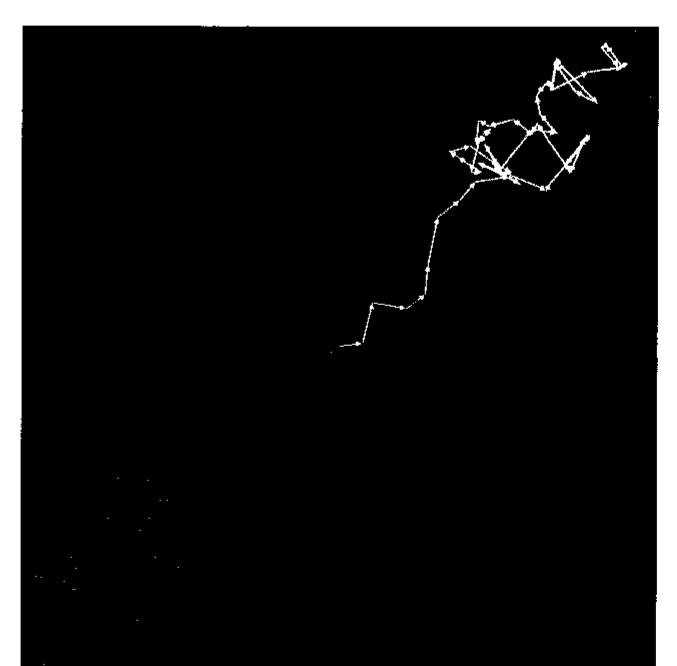
\includegraphics[width=0.5\textwidth]{ch20-fig20-6-langevin.png}
  \caption{使用\eqref{align:ch14-langevin更新}定义的 Langevin 动力学得到的采样轨迹，这里显示了三条都从图中心开始的采样轨迹（参见\cref{section:ch14-langevin采样}）}
  \label{figure:ch20-Langevin}
\end{figure}

\subsection{噪声方差}\label{subsection:ch20-噪声方差}

我们已经了解怎么从一组训练数据中学习得分函数，以及如何使用 Langevin 动力学方法从学习到的分布中进行采样并生成新的样本。然而，这种方法存在三个潜在的问题（Song and Ermon, 2019; Luo, 2022）（参见\cref{chapter:ch16-连续潜变量}）。第一，如果数据分布位于比数据空间维度更低的流形上，那么流形之外的点的概率密度将为零，此时因为 $\ln p(\bm{x})$ 是未定义的，所以得分函数是未定义的。第二，在数据密度低的区域，得分函数的估计可能不准确，因为损失函数\eqref{align:ch20-得分损失}被密度加权了。一个不准确的得分函数会导致使用 Langevin 动力学方法采样时轨迹不佳。第三，即使有一个准确的得分函数，如果数据分布包括一系列不连续的混合分布，通过 Langevin 动力学方法也可能无法正确采样（见\cref{exercise:ch20-18}）。

以上三个问题都可以通过选择核函数\eqref{align:ch20-Gauss核}中使用的噪声方差 $\sigma^2$ 的足够大值来解决，因为这会使数据分布平滑。然而，过大的方差会导致原始分布显著失真，导致得分函数建模失准。一个折中方案是引入方差序列 $\sigma_1^2<\sigma_2^2<\cdots<\sigma_L^2$（Song and Ermon, 2019），其中 $\sigma_1^2$ 足够小，以便数据分布得到准确表示；而 $\sigma_L^2$ 则足够大，以避免上述问题。然后修改得分网络，使其将方差作为额外的输入 $\bm{s}(\bm{x},\bm{w},\sigma^2)$，并通过使用一个加权和形式的损失函数\eqref{align:ch20-经验损失}对其进行训练，其中的每一项表示相关网络与相应扰动数据集之间的误差。对于数据向量 $\bm{x}_n$，损失函数的形式为
\begin{align}
\frac{1}{2}\sum_{i=1}^{L}\lambda(i)\int\big\|\bm{s}(\bm{z},\bm{w},\sigma_i^2)-\nabla_{\bm{z}}\ln q(\bm{z}\mid\bm{x}_n,\sigma_i)\big\|^2q(\bm{z}\mid\bm{x}_n,\sigma_i)\,\mathrm{d}\bm{z},
\label{align:ch20-退火损失}
\end{align}
其中 $\lambda(i)$ 是权重系数。这个训练过程精确地对应于用来训练分层去噪网络的机制（参见\cref{subsection:ch20-训练解码器}）。

训练完成后，可以通过依次对 $i=L,L-1,\cdots,2,1$ 的每个模型逐个执行几步 Langevin 动力学方法进行采样并生成样本。这种技术称为\textbf{退火 Langevin 动力学}（annealed Langevin dynamics），类似于用来从去噪扩散概率模型中采样的算法 20.2。

\subsection{随机微分方程}\label{subsection:ch20-随机微分方程}

在构建扩散模型的加噪过程时，使用大数量的步骤（通常为几千步）是有益处的。因此，我们需要考虑在无穷步数的极限情况下会发生什么，就像我们在引入神经微分方程时为无限深度的神经网络所做的那样（参见\cref{section:ch18-连续流}）。在这种极限情况下，我们需要确保每一步的噪声方差 $\beta_t$ 随着步长变小而同步变小。这引出了连续时间下扩散模型的理论框架，即\textbf{随机微分方程}（Stochastic Differential Equation, SDE）（Song et al., 2020）。去噪扩散概率模型和得分匹配模型都可以视为连续时间 SDE 的离散化实现。

我们可以将一般的 SDE 写成向量 $\bm{z}$ 的无穷小更新：
\begin{align}
\mathrm{d}\bm{z}=\underbrace{\bm{f}(\bm{z},t)\,\mathrm{d}t}_{\text{漂移项}}+\underbrace{g(t)\,\mathrm{d}\bm{w}}_{\text{扩散项}},
\label{align:ch20-SDE}
\end{align}
其中漂移项（drift term）是确定性的，类似于常微分方程（ODE），但扩散项（diffusion term）是随机的。这里的参数 $t$ 常常称为“时间”，类比于物理系统中的时间。扩散模型的前向加噪过程\eqref{align:ch20-递推}，可以通过采取连续时间极限而写成形如\eqref{align:ch20-SDE}的 SDE（见\cref{exercise:ch20-19}）。

\begin{definition}[随机微分方程]\label{definition:ch20-随机微分方程}
设 $\bm{f}(\bm{z},t)$ 为漂移系数、$g(t)$ 为扩散系数、$\bm{w}$ 为标准 Wiener 过程。称形如\eqref{align:ch20-SDE}的方程为 \textbf{It\^o 随机微分方程}（SDE），其解 $\bm{z}(t)$ 是一个连续时间的随机过程：$\bm{f}$ 描述确定性的漂移，$g\,\mathrm{d}\bm{w}$ 描述随机的扩散。
\end{definition}

% SUPPLEMENT: parent=definition:ch20-随机微分方程; kind=motivation; location=紧随其后的 remark（重构新增）
\begin{remark}（重构新增）
SDE 可以看作“常微分方程 + 噪声”的连续时间极限：把 $\mathrm{d}\bm{w}$ 理解为均值为零、方差为 $\mathrm{d}t$ 的 Gauss 增量，就回到了离散的更新式。它之所以适合描述扩散模型，是因为前向加噪过程的步数 $T$ 可以趋于无穷，而每一步的方差 $\beta_t$ 必须随步长同步缩小，否则极限不存在。\par
记号上要注意两点：其一，这里写的是 It\^o 形式，$g\,\mathrm{d}\bm{w}$ 的积分按 It\^o 定义，因而普通微积分的链式法则需要换成 It\^o 公式；其二，$g$ 只依赖 $t$ 而不依赖 $\bm{z}$，这是本书的简化约定，一般的 SDE 允许 $g(\bm{z},t)$。\par
条件：$\bm{f}$ 关于 $\bm{z}$ 满足 Lipschitz 条件、$g$ 有界，才能保证 SDE 有唯一强解；若这些条件不满足，解可能在有限时间爆炸，后面的 Fokker--Planck 论证也随之失效。
\end{remark}

对于 SDE\eqref{align:ch20-SDE}，存在一个对应的逆向 SDE（Song et al., 2020），如下所示：
\begin{align}
\mathrm{d}\bm{z}=\big\{\bm{f}(\bm{z},t)-g^2(t)\nabla_{\bm{z}}\ln p_t(\bm{z})\big\}\,\mathrm{d}t+g(t)\,\mathrm{d}\bar{\bm{w}},
\label{align:ch20-逆SDE}
\end{align}
其中 $\nabla_{\bm{z}}\ln p_t(\bm{z})$ 是得分函数。对于\eqref{align:ch20-SDE}给出的 SDE，应从 $t=T$ 倒序求解至 $t=0$。

对于所有由 SDE 支配的扩散过程，都存在一个相应的由 ODE 描述的确定性过程，其轨迹具有与 SDE 相同的边缘概率密度 $p_t(\bm{z})$（Song et al., 2020）。对于形如\eqref{align:ch20-SDE}的 SDE，相应的 ODE 为
\begin{align}
\frac{\mathrm{d}\bm{z}}{\mathrm{d}t}=\bm{f}(\bm{z},t)-\frac{1}{2}g^2(t)\nabla_{\bm{z}}\ln p_t(\bm{z}).
\label{align:ch20-ODE}
\end{align}

\begin{proposition}[逆时 SDE 与概率流 ODE]\label{proposition:ch20-逆时SDE}
设 $p_t$ 是\eqref{align:ch20-SDE}的解的密度，关于 $t$ 连续可微、关于 $\bm{z}$ 二阶连续可微，在无穷远处充分快衰减，并满足 Fokker--Planck 方程
\begin{align*}
\frac{\partial p_t}{\partial t}=-\nabla_{\bm{z}}\cdot\big(\bm{f}(\bm{z},t)p_t\big)+\frac{1}{2}g^2(t)\Delta_{\bm{z}}p_t.
\end{align*}
则：(i) 逆向 SDE\eqref{align:ch20-逆SDE}从 $t=T$ 倒序求解时，其边缘密度为 $p_t$；(ii) ODE\eqref{align:ch20-ODE}的轨道具有与\eqref{align:ch20-SDE}相同的边缘密度 $p_t$。
\end{proposition}

\begin{proof}（重构新增）
先证 (ii)。令 $\bm{v}(\bm{z},t)=\bm{f}(\bm{z},t)-\frac{1}{2}g^2(t)\nabla_{\bm{z}}\ln p_t(\bm{z})$，则 $\bm{v}p_t=\bm{f}p_t-\frac{1}{2}g^2\nabla_{\bm{z}}p_t$，取散度得
\begin{align*}
\nabla_{\bm{z}}\cdot(\bm{v}p_t)=\nabla_{\bm{z}}\cdot(\bm{f}p_t)-\frac{1}{2}g^2\Delta_{\bm{z}}p_t.
\end{align*}
而由 Fokker--Planck 方程，$\partial_tp_t=-\nabla_{\bm{z}}\cdot(\bm{f}p_t)+\frac{1}{2}g^2\Delta_{\bm{z}}p_t=-\nabla_{\bm{z}}\cdot(\bm{v}p_t)$。这正是连续性方程，故 ODE $\mathrm{d}\bm{z}/\mathrm{d}t=\bm{v}(\bm{z},t)$ 精确输运密度 $p_t$：其轨道的边缘密度在任意 $t$ 都等于 $p_t$。
再证 (i)。令 $\tau=T-t$，$q_{\tau}(\bm{z})=p_{T-\tau}(\bm{z})$。把\eqref{align:ch20-逆SDE}按反时方向记为 $\tau$ 增加方向的 SDE，其漂移为 $-\big\{\bm{f}-g^2\nabla\ln p\big\}$、扩散系数仍为 $g$。由 Fokker--Planck 方程，$q_{\tau}$ 满足
\begin{align*}
\frac{\partial q_{\tau}}{\partial\tau}&=-\nabla_{\bm{z}}\cdot\Big(\big(-\bm{f}+g^2\nabla_{\bm{z}}\ln q_{\tau}\big)q_{\tau}\Big)+\frac{1}{2}g^2\Delta_{\bm{z}}q_{\tau}\\
&=\nabla_{\bm{z}}\cdot(\bm{f}q_{\tau})-g^2\Delta_{\bm{z}}q_{\tau}+\frac{1}{2}g^2\Delta_{\bm{z}}q_{\tau}=\nabla_{\bm{z}}\cdot(\bm{f}q_{\tau})-\frac{1}{2}g^2\Delta_{\bm{z}}q_{\tau}.
\end{align*}
另一方面，由 $q_{\tau}=p_{T-\tau}$ 与 Fokker--Planck 方程，$\partial_{\tau}q_{\tau}=-\partial_tp_t|_{T-\tau}=\nabla_{\bm{z}}\cdot(\bm{f}q_{\tau})-\frac{1}{2}g^2\Delta_{\bm{z}}q_{\tau}$。两式相同，故 $q_{\tau}$ 就是逆时 SDE 的密度，即逆时 SDE 的边缘密度为 $p_{T-\tau}$；换回 $t$ 即得 (i)。证毕。
\end{proof}

% SUPPLEMENT: parent=proposition:ch20-逆时SDE; kind=motivation; location=紧随其后的 remark（重构新增）
\begin{remark}（重构新增）
这条命题是“连续时间扩散模型”的理论核心：它把“加噪—去噪”的离散图像换成了“一个 SDE 与其逆时 SDE 具有相同边缘分布”的连续图像。证明只用到 Fokker--Planck 方程与连续性方程，两条方程分别刻画“随机过程的密度演化”与“确定性流对密度的输运”，因此结论是精确的，而非近似。\par
ODE\eqref{align:ch20-ODE}称为概率流 ODE（probability flow ODE），它的轨道是确定性的：给定初值 $\bm{z}_T$，整条轨迹就被确定，因而它定义了从先验到数据的可逆映射，可以把扩散模型与标准化流联系起来，用变量替换公式精确计算对数似然（参见\cref{section:ch18-连续流}）。\par
条件不能省：$p_t$ 的光滑性与衰减性保证 Fokker--Planck 方程的分部积分合法；$\nabla_{\bm{z}}\ln p_t$ 必须存在，否则逆时 SDE 的漂移无定义。逆时 SDE 中的 $\mathrm{d}\bar{\bm{w}}$ 是反向时间轴上的 Wiener 增量，它把“时间的箭头”翻转过来——这正是从 $t=T$ 倒序求解的含义。
\end{remark}

要想数值求解 SDE，我们需要对时间变量进行离散化。最简单的方法是使用固定且等间距的时间步，这称为 Euler--Maruyama 求解器。对于反向 SDE，我们可以先恢复 Langevin 方程的一种形式（参见\cref{section:ch14-langevin采样}），再采用更复杂的求解器，这些求解器使用了更灵活的离散化形式（Kloeden and Platen, 2013）。

该 ODE 允许使用高效的自适应步长求解器以最大限度地减少函数评估次数。此外，ODE 还允许将概率扩散模型与标准化流模型相关联，后者允许使用变量替换\eqref{align:ch18-change-var}来精确计算对数似然（参见\cref{section:ch18-连续流}）。

\end{document}
